\subsection{Results on STR-MF} \label{experimental_results_spatial}
Here we focus on Berkeley data set because only in which the location information of sensor nodes is available. 

\begin{table} [htbp]
\caption{RMSE of Berkeley Random split} \label{table:spatial_random}
\setlength{\tabcolsep}{2pt}
\centering
\small
\begin{tabular} {c | r r r | r r r | r r r}
& \multicolumn{3}{ c|}{Humidity} & \multicolumn{3}{|c|}{Light} & \multicolumn{3}{|c }{Temperature} \\ \hline
train & \begin{turn}{65}TR-MF\end{turn} & \begin{turn}{65}STR-MF\end{turn} & \begin{turn}{65}sTR-MF\end{turn}& \begin{turn}{65}TR-MF\end{turn} & \begin{turn}{65}STR-MF\end{turn} & \begin{turn}{65}sTR-MF\end{turn}& \begin{turn}{65}TR-MF\end{turn} & \begin{turn}{65}STR-MF\end{turn} & \begin{turn}{65}sTR-MF\end{turn} \\ \hline
10\% & $ \mathbf{ 0.142 } $ & $ 0.484 $ & $ 0.173 $ & $ \mathbf{ 35.5 } $ & $ 97.4 $ & $ 38.3 $ & $ \mathbf{ 0.046 } $ & $ 0.154 $ & $ 0.061 $\\
20\% & $ \mathbf{ 0.114 } $ & $ 0.424 $ & $ 0.135 $ & $ \mathbf{ 28.2 } $ & $ 90.6 $ & $ 28.9 $ & $ \mathbf{ 0.032 } $ & $ 0.146 $ & $ 0.047 $\\
40\% & $ \mathbf{ 0.092 } $ & $ 0.352 $ & $ 0.104 $ & $ \mathbf{ 21.2 } $ & $ 85.8 $ & $ 22.8 $ & $ \mathbf{ 0.023 } $ & $ 0.145 $ & $ 0.037 $\\
60\% & $ \mathbf{ 0.082 } $ & $ 0.337 $ & $ 0.093 $ & $ \mathbf{ 17.2 } $ & $ 83.3 $ & $ 18.3 $ & $ \mathbf{ 0.018 } $ & $ 0.147 $ & $ 0.031 $\\
80\% & $ \mathbf{ 0.076 } $ & $ 0.324 $ & $ 0.084 $ & $ \mathbf{ 17.7 } $ & $ 84.4 $ & $ 18.1 $ & $ \mathbf{ 0.015 } $ & $ 0.148 $ & $ 0.027 $\\
85\% & $ \mathbf{ 0.075 } $ & $ 0.326 $ & $ 0.083 $ & $ \mathbf{ 14.4 } $ & $ 82.0 $ & $ 15.8 $ & $ \mathbf{ 0.016 } $ & $ 0.138 $ & $ 0.028 $\\
\end{tabular}
\end{table}

\begin{table} [htbp]
\caption{RMSE of Berkeley Temporal split} \label{table:spatial_temporal}
\setlength{\tabcolsep}{2pt}
\centering
\small
\begin{tabular} {c | r r r | r r r | r r r}
& \multicolumn{3}{ c|}{Humidity} & \multicolumn{3}{|c|}{Light} & \multicolumn{3}{|c }{Temperature} \\ \hline
train & \begin{turn}{65}TR-MF\end{turn} & \begin{turn}{65}STR-MF\end{turn} & \begin{turn}{65}sTR-MF\end{turn}& \begin{turn}{65}TR-MF\end{turn} & \begin{turn}{65}STR-MF\end{turn} & \begin{turn}{65}sTR-MF\end{turn}& \begin{turn}{65}TR-MF\end{turn} & \begin{turn}{65}STR-MF\end{turn} & \begin{turn}{65}sTR-MF\end{turn} \\ \hline
10\% & $ 0.957 $&$ 0.573 $&$ \mathbf{ 0.547 } $&$ \mathbf{ 220.070 } $&$ 281.607 $&$ 264.763 $&$ 0.515 $&$ \mathbf{ 0.242 } $&$ 0.307 $\\
20\% & $ 0.796 $&$ 0.657 $&$ \mathbf{ 0.459 } $&$ \mathbf{ 113.310 } $&$ 236.865 $&$ 230.054 $&$ 0.392 $&$ \mathbf{ 0.179 } $&$ 0.187 $\\
40\% & $ 0.771 $&$ 0.520 $&$ \mathbf{ 0.455 } $&$ \mathbf{ 58.090 } $  & $ 110.758 $ &  $ 64.388 $&$ 0.310 $&$ 0.196 $&$ \mathbf{ 0.189 } $\\
60\% & $ 0.540 $&$ \mathbf{ 0.351 } $&$ 0.708 $&$ \mathbf{ 41.730 } $  & $ 150.149 $ &  $ 69.235 $&$ 0.206 $&$ \mathbf{ 0.191 } $&$ 0.243 $\\
80\% & $ 0.447 $&$ 0.299 $&$ \mathbf{ 0.261 } $&$ \mathbf{ 21.450 } $  & $ 112.694 $ &  $ 28.017 $&$ 0.132 $&$ \mathbf{ 0.108 } $&$ 0.114 $\\
85\% & $ 0.323 $&$ \mathbf{ 0.166 } $&$ 0.256 $&$ \mathbf{ 8.310 } $   & $ 85.423 $  &  $ 12.079 $&$ 0.088 $&$ \mathbf{ 0.065 } $&$ 0.082 $\\
\end{tabular}
\end{table}



%Table \ref{table:spatial_random_hum}, \ref{table:spatial_random_light}, \ref{table:spatial_random_tem}, \ref{table:spatial_temporal_hum}, \ref{table:spatial_temporal_light}, \ref{table:spatial_temporal_tem}  show the result of adding spatial regularization. 
Table \ref{table:spatial_random} and \ref{table:spatial_temporal} compare STF-MF with TR-MF.
STR-MF mean TR-MF with strong spatial regularization, while sTR-MF is with weak spatial regularization. We got no improvement in all random split data and either (temporal, light). However, we see significant improvement on (temporal, humidity) and (temporal, temperature).

There are two factors that decide the successfulness of spatial regularization. 
On the one hand, TR-MF already captures some of the spatial correlation. 
Since we have thousands of readings for every sensor node, TR-MF can learn the spatial correlation from the data and create similar factors for similar sensor nodes. 
On the other hand, the neighboring pairs in the deployment graph may not imply the actual similarity.
For example, we can look at the similarity graph of humidity and light sensors.
We define the similarity of sensor node $n_i$ and $n_j$ as by the factor similarity:
%\begin{equation*}
$\frac{q_{n_i}^T q_{n_j}}{max(||q_{n_i}||^2, ||q_{n_j}||^2)},$
%\end{equation*}
and we get the similarity graph:
\begin{figure}[ftbp]
\centering
\subfigure[Expected Similarity]{
	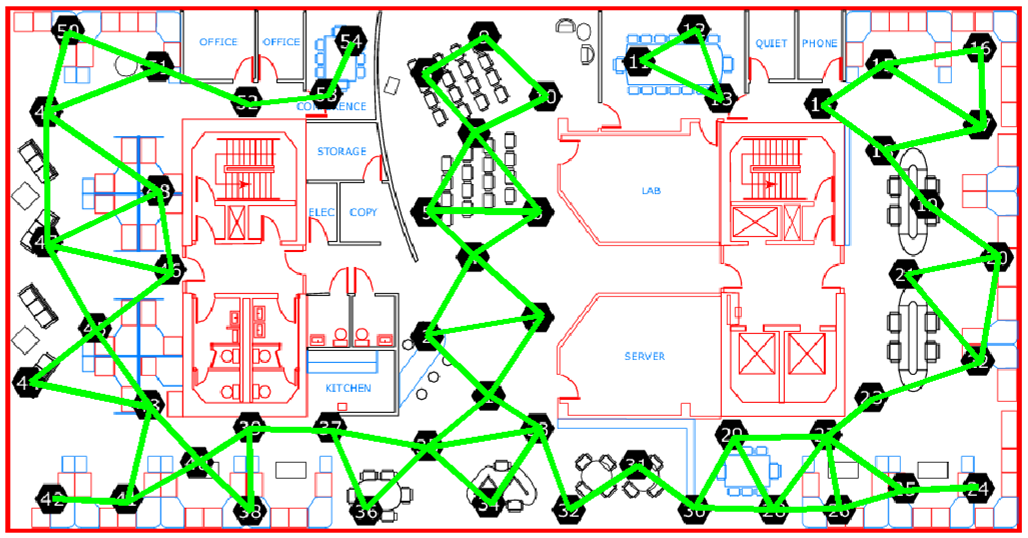
\includegraphics[width=0.25\textwidth]{expected.png}
}\\
\subfigure[Humidity: top 100 similar pairs]{
	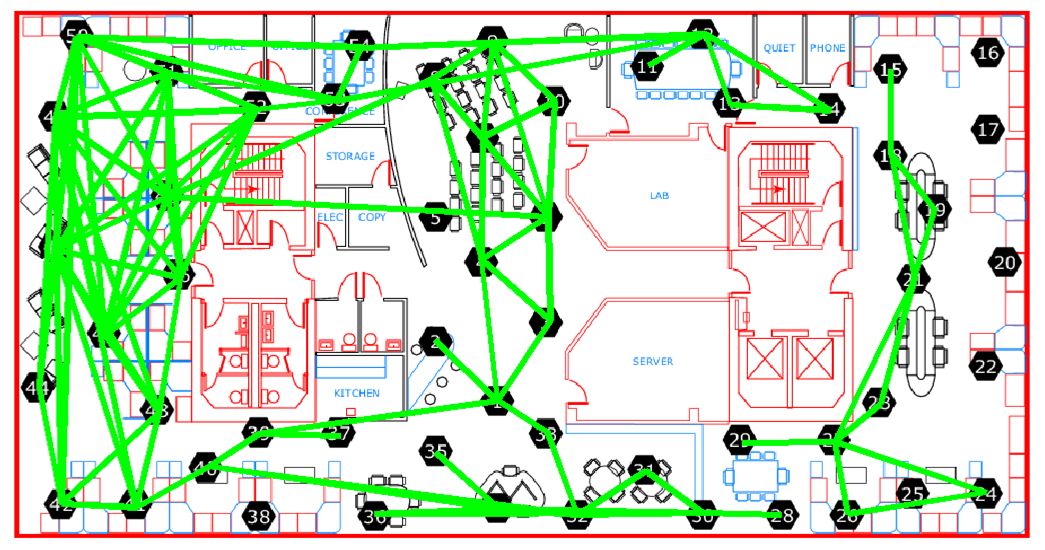
\includegraphics[width=0.22\textwidth]{Hum_similarity.png}
}
\hspace{0in}
\subfigure[Light: top 100 similar pairs]{
	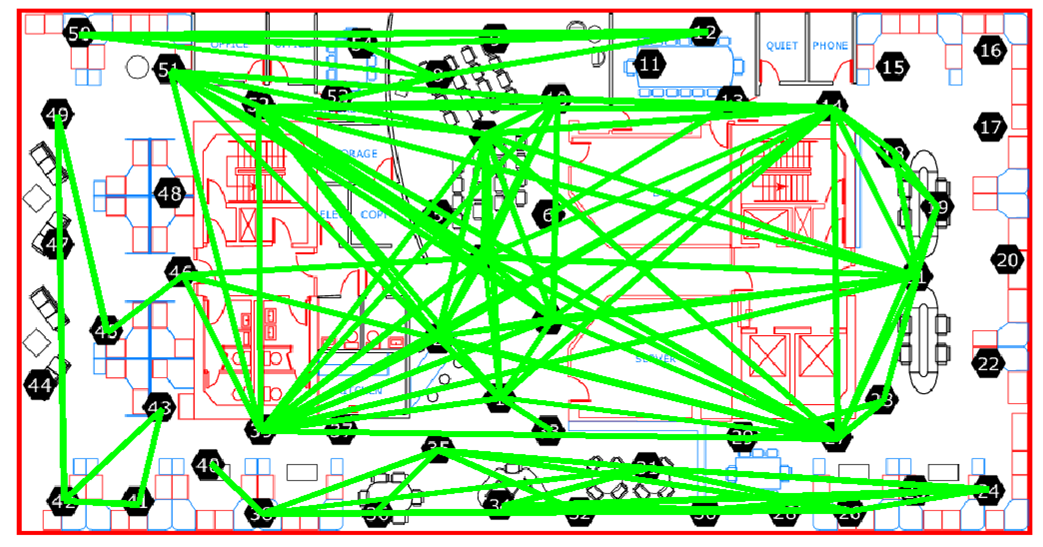
\includegraphics[width=0.22\textwidth]{Light_similarity.png}
}
\end{figure}

We can see that the similarity graph of humidity is more similar to our expectation, while the similarity graph of light is not. We can only obtain improvement when the data information is insufficient, which is the temporal split case, and when our expectation similarity is not far from the actual similarity, which is the temperature and humidity.

